\documentclass[tikz,border=10pt]{standalone}
\usepackage{tikz}
\usetikzlibrary{shapes,arrows,positioning,fit,backgrounds}

\begin{document}
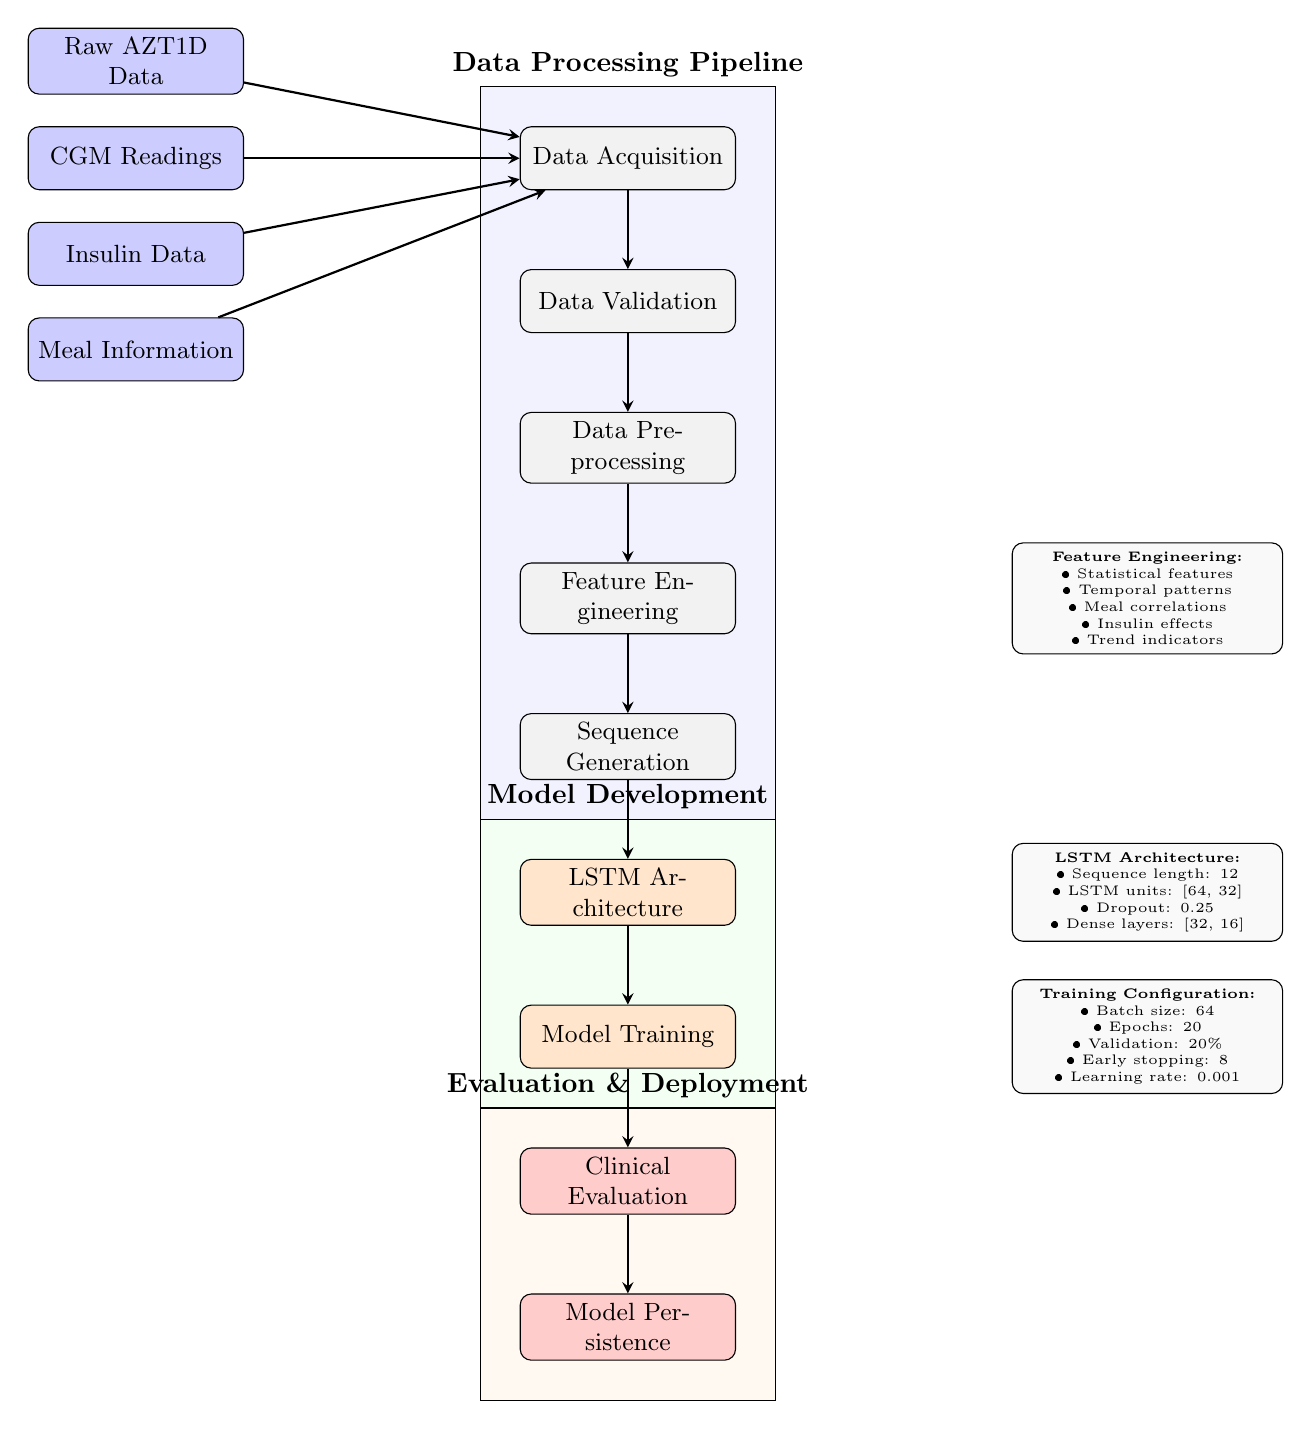
\begin{tikzpicture}[
    node distance=1.5cm,
    data/.style={rectangle, draw, fill=blue!20, text width=2.5cm, text centered, minimum height=0.8cm, rounded corners, font=\small},
    process/.style={rectangle, draw, fill=green!20, text width=2.5cm, text centered, minimum height=0.8cm, rounded corners, font=\small},
    model/.style={rectangle, draw, fill=orange!20, text width=2.5cm, text centered, minimum height=0.8cm, rounded corners, font=\small},
    output/.style={rectangle, draw, fill=red!20, text width=2.5cm, text centered, minimum height=0.8cm, rounded corners, font=\small},
    arrow/.style={thick,->,>=stealth},
    stage/.style={rectangle, draw, fill=gray!10, text width=2.5cm, text centered, minimum height=0.8cm, rounded corners, font=\small},
    config/.style={rectangle, draw, fill=gray!5, text width=3.2cm, text centered, minimum height=1.2cm, rounded corners, font=\tiny}
]

% Data Sources (left column)
\node[data] (raw) {Raw AZT1D Data};
\node[data, below=0.4cm of raw] (cgm) {CGM Readings};
\node[data, below=0.4cm of cgm] (insulin) {Insulin Data};
\node[data, below=0.4cm of insulin] (meals) {Meal Information};

% Pipeline stages (center column)
\node[stage, right=3.5cm of cgm] (acquisition) {Data Acquisition};
\node[stage, below=1cm of acquisition] (validation) {Data Validation};
\node[stage, below=1cm of validation] (preprocessing) {Data Preprocessing};
\node[stage, below=1cm of preprocessing] (features) {Feature Engineering};
\node[stage, below=1cm of features] (sequences) {Sequence Generation};
\node[model, below=1cm of sequences] (lstm) {LSTM Architecture};
\node[model, below=1cm of lstm] (training) {Model Training};
\node[output, below=1cm of training] (evaluation) {Clinical Evaluation};
\node[output, below=1cm of evaluation] (persistence) {Model Persistence};

% Configuration details (right column)
\node[config, right=3.5cm of features] (feat_config) {
    \textbf{Feature Engineering:}\\
    • Statistical features\\
    • Temporal patterns\\
    • Meal correlations\\
    • Insulin effects\\
    • Trend indicators
};

\node[config, right=3.5cm of lstm] (lstm_config) {
    \textbf{LSTM Architecture:}\\
    • Sequence length: 12\\
    • LSTM units: [64, 32]\\
    • Dropout: 0.25\\
    • Dense layers: [32, 16]
};

\node[config, right=3.5cm of training] (train_config) {
    \textbf{Training Configuration:}\\
    • Batch size: 64\\
    • Epochs: 20\\
    • Validation: 20\%\\
    • Early stopping: 8\\
    • Learning rate: 0.001
};

% Arrows from data sources to acquisition
\draw[arrow] (raw) -- (acquisition);
\draw[arrow] (cgm) -- (acquisition);
\draw[arrow] (insulin) -- (acquisition);
\draw[arrow] (meals) -- (acquisition);

% Pipeline flow (vertical)
\draw[arrow] (acquisition) -- (validation);
\draw[arrow] (validation) -- (preprocessing);
\draw[arrow] (preprocessing) -- (features);
\draw[arrow] (features) -- (sequences);
\draw[arrow] (sequences) -- (lstm);
\draw[arrow] (lstm) -- (training);
\draw[arrow] (training) -- (evaluation);
\draw[arrow] (evaluation) -- (persistence);

% Add background boxes for pipeline stages
\begin{scope}[on background layer]
    \node[fit=(acquisition) (validation) (preprocessing) (features) (sequences), 
          draw, fill=blue!5, inner sep=0.5cm, label=above:\textbf{Data Processing Pipeline}] {};
    \node[fit=(lstm) (training), 
          draw, fill=green!5, inner sep=0.5cm, label=above:\textbf{Model Development}] {};
    \node[fit=(evaluation) (persistence), 
          draw, fill=orange!5, inner sep=0.5cm, label=above:\textbf{Evaluation \& Deployment}] {};
\end{scope}

\end{tikzpicture}
\end{document}
